\subsection{Fill holes}

Om betrouwbaar een object te kunnen identificeren vullen we de gaten op in de
objecten. Deze gaten kunnen ontstaan zijn bij de RGB filtering door schittering
op het object.

Het proces om de gaten te vullen is relatief eenvoudig. Door de achtergrond te
markeren en vervolgens alle niet gemarkeerde pixels op 1 te zetten is het vullen
voltooid. Om een start te maken voor het markeren van de achtergrond is het
mogelijk om alle rand pixels die 0 zijn te markeren als, bijvoorbeeld, een 2
(figuur \ref{fig:fhstep1}). Dit zal op een zelfde wijze gaan als bij de remove
border blobs operator.

Omdat enkel de rand gescand hoeft te worden kan deze functie redelijk snel
uitgevoerd worden (listing \ref{list:mark-non-blob-borders}). Het voltooien van
de pixel scan wordt op dezelfde manier gedaan als beschreven bij de remove
border blobs operatie (sectie \ref{sec:remove-border}). Vanuit alle gemarkeerde
pixels wordt er voortborduurt tot het hele plaatje is gemarkeerd. In dit geval
mag er dus geen 2-0 bij x connected overgang meer zijn. Tot slot moeten alle
pixels gemarkeerd met 0 gemarkeerd worden als een 1. Daarna worden de pixels
gemarkeerd met 2, gemarkeerd als een 0. Helaas gaat dit niet in 1 stap omdat
anders het hele plaatje gemarkeerd wordt als 1 (figuur \ref{fig:fhstep4}).

\begin{listing}
    \begin{minted}{c}
    for(w = width; w >= 0; w--){
        if(imgArr[0][w] == 0){
            imgArr[0][w] = 2;
        }
        if(imgArr[height][w] == 0){
            imgArr[height][w] = 2;
        }
    }
    \end{minted}
    \caption{Markeren van rand pixels die geen onderdeel uitmaken van een blob}
    \label{list:mark-non-blob-borders}
\end{listing}

\begin{figure}
    \begin{center}
        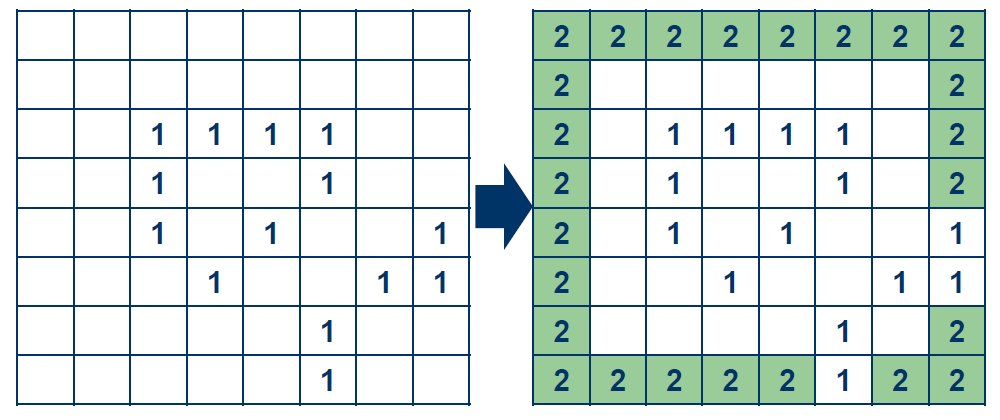
\includegraphics[scale=0.35]{figures/fill_holes_step1.png}
    \end{center}
    \caption{Achtergrond rand markeren.}
    \label{fig:fhstep1}
\end{figure}

\begin{figure}
    \begin{center}
        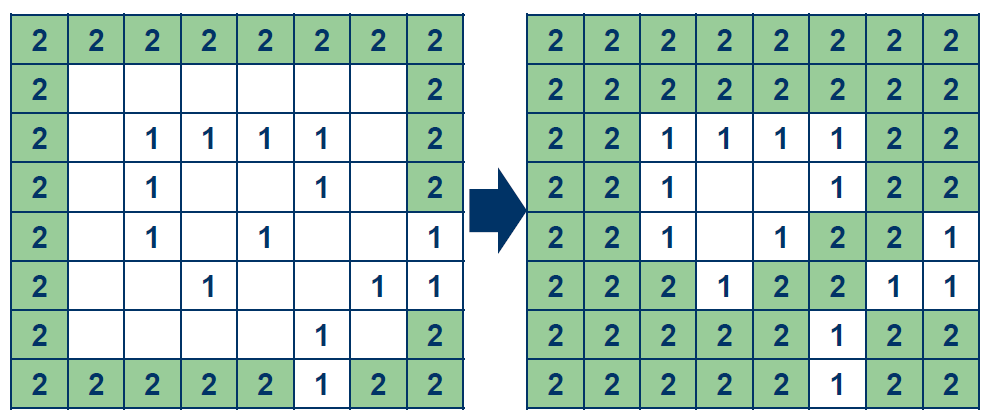
\includegraphics[scale=0.35]{figures/fill_holes_step2.png}
    \end{center}
    \caption{Achtergrond rand markeren}
    \label{fig:fhstep2}
\end{figure}

\begin{figure}
    \begin{center}
        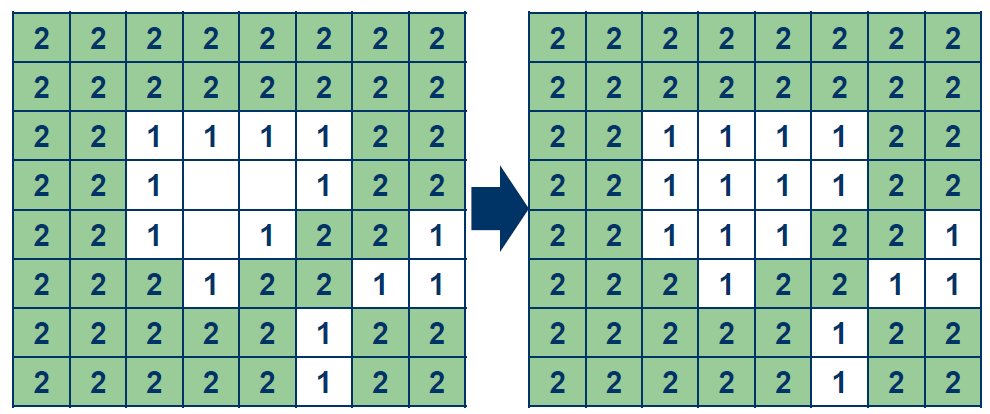
\includegraphics[scale=0.35]{figures/fill_holes_step3.png}
    \end{center}
    \caption{Blobs inkleuren}
    \label{fig:fhstep3}
\end{figure}

\begin{figure}
    \begin{center}
        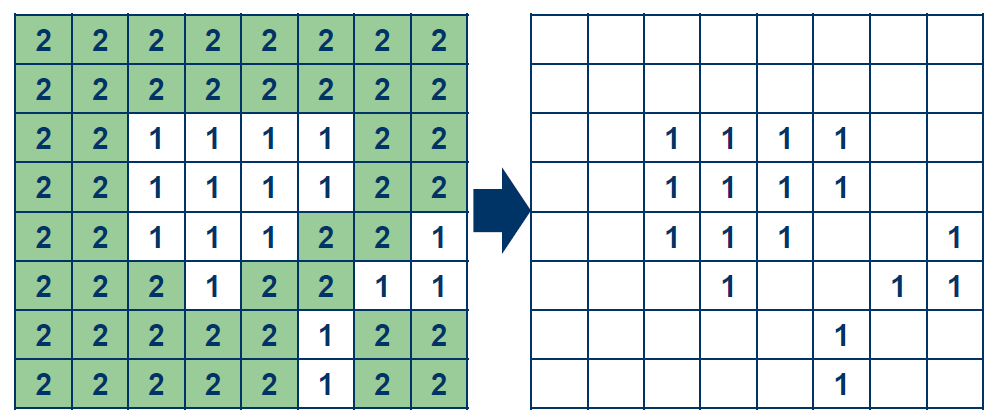
\includegraphics[scale=0.35]{figures/fill_holes_step4.png}
    \end{center}
    \caption{Achtergrond weer 0 maken}
    \label{fig:fhstep4}
\end{figure}
